
\paragraph{Imperfection field implementation}\label{chpt3:imperfections:implementation}
When implementing machine imperfections we followed recommendations given in~\cite[p.~235]{Eremey:Thesis}. 
A small perturbation of the magnetic field acts like a proportional rotation of the spin vector.
For this reason we implemented the E+B element tilt as a product between the element's spin transfer matrix
and the corresponding rotation matrix, a ``spin kick.'' Such an implementation guarantees the preservation of 
the closed orbit. This orbit preservation is physically grounded in the fact that when a spin-rotator
is tilted, there emerges a compensating electric field keeping the Lorentz force constant.

According to equation~\eqref{eq:TBMT_MDM}, a change in the MDM precession angular velocity
associated with the presence of a parasitic magnetic field $(B_x, 0, B_z)$ is
\begin{align*}
	\Delta\W_{MDM} &= \frac qm G \cdot (B_x, 0, B_z),
	\intertext{hence the spin kick angle}
	\Theta_{kick} &= t_0\Delta\W_{MDM},
\end{align*}
where $t_0 = L/v_0$ is the reference particle's time of flight through the element.

\subsection{Tilt distribution dependence} \label{chpt3:imperfections:magnitude}
This series of simulations was carried out in order to prove (or reject) the validity of two theses
concerning the machine imperfection systematic error:
\begin{enumerate*}[(1)]
	\item the induced MDM spin precession angular velocity component is independent of the particular
	element tilt distribution, and depends only on the mean tilt angle; and
	\item this dependence is linear.
\end{enumerate*}

The simulation was set up as follows: in the FS lattice described in section~\ref{chpt2:lattice:FS_BNL} 
 E+B elements were randomly tilted about the optic axis by angles $\Theta_{tilt}$.
 After building the third-order spin and orbital transfer maps, we computed the Taylor expansions of the
 spin tune and spin precession axis (SPA). The zero-order terms of the Taylor expansions represent the spin tune and SPA
 of the reference particle.
 
 The reference particle spin precession angular velocity is calculated 
 according to equation:~\cite[p.~4]{COSY:SpinTuneMapping}
\[
\vec\W = 2\pi/\tau_0\cdot \nu_s \cdot \bar n,
\]
where $\tau_0 = f^{-1}_{rev} = 10^{-6}$ seconds is the particle's time of flight through the full lattice.

The simulation was carried out 11 times; each time the spin-rotator tilt angles were picked
from a normal distribution $N(\mu_0\cdot(i-5), \sigma_0)$, where 
$\mu_0 = 10\cdot \sigma_0 = 10^{-4}$ rad, $i\in\lbrace0,\dots, 10\rbrace$. The simulation
results are plotted in Figure~\ref{fig:Linearity_test_shifting_gauss}.

\begin{figure}[!h]
	\centering
	\begin{subfigure}{\linewidth}
		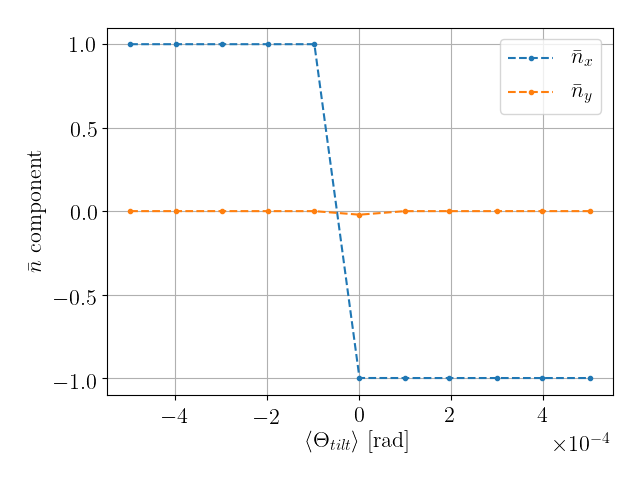
\includegraphics[height=.35\paperheight]{images/fake_signal_sim/linearity_test_shifting_gauss_nbar}
		\caption{Spin precession axis $\nbar$ components.}
	\end{subfigure}
	\begin{subfigure}{\linewidth}
		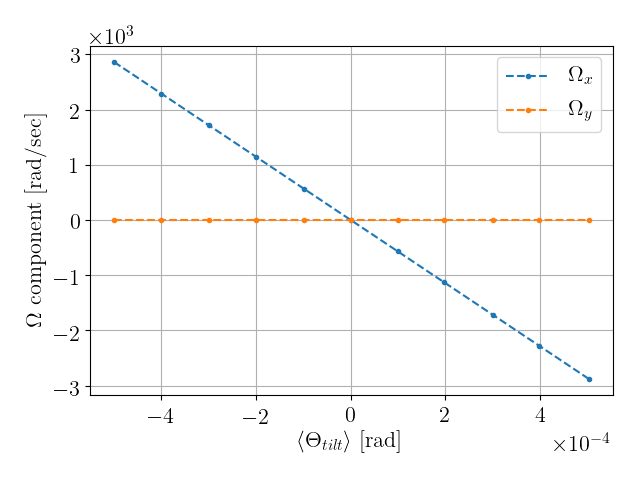
\includegraphics[height=.35\paperheight]{images/fake_signal_sim/linearity_test_shifting_gauss_freq}
		\caption{Angular velocity $\vec\W$ components.}
	\end{subfigure}
	\caption{Reference particle's spin precession axis and angular velocity components as
		 functions of the mean E+B element tilt angle. Element tilts are normally distributed.
		Color identifies the component; radial (blue) and vertical (orange).\label{fig:Linearity_test_shifting_gauss}}
\end{figure}

One can observe from the figure that a tilt distribution at which the mean tilt angle is equal to $10^{-4}$ radians, the
beam polarization vector precesses in the vertical plane at the rate of 500 rad/sec. This agrees with the estimates
mentioned above (section~\ref{chpt3:imperfections}), because in them a tilt error standard deviation of $10^{-4}$ rad 
is assumed at 100 tilted elements. In that case, the mean tilt angle standard deviation is $10^{-5}$, and hence MDM
precession occurs at a rate up to 50 rad/sec with a probability 67\%, and up to 100 rad/sec with a probability 95\%.

Figure~\ref{fig:Linearity_test_compensated} shows the results of a simulation in which six randomly-picked
E+B elements were pair-wise tilted by opposite angles, while one element was tilted by an angle
$\mu_i = (i-5)\cdot 10^{-6}$ rad, $i\in\lbrace0,\dots,10\rbrace$. 

Both simulations were done at the strict FS energy 270.0092 MeV.\footnote{At this energy, in the ideal lattice, 
	$\nu_s$ and $\nbar$	are undefined in the beam rest frame used in COSY Infinity.
	This corresponds to the situation when spin does not precess in any plane (either horizontal or vertical), 
	which corresponds to the realization of the 3D FS condition in an ideal lattice.} One can see that the compensated
elements do not contribute to the spin precession.

\begin{figure}[!h]
	\centering
	\begin{subfigure}{\linewidth}
		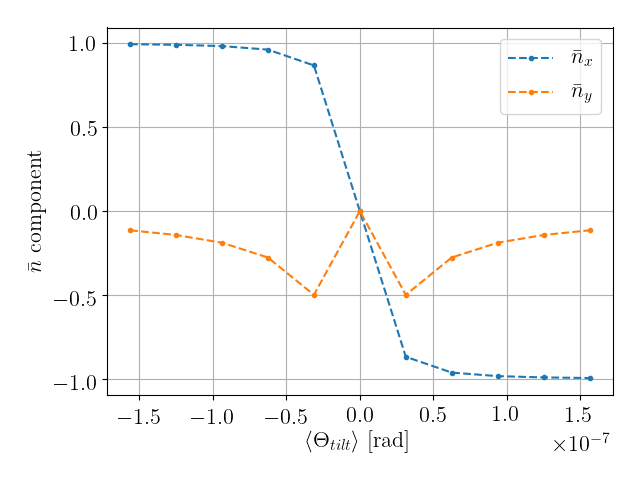
\includegraphics[height=.35\paperheight]{images/fake_signal_sim/linearity_test_compensated+microrad_nbar}
		\caption{Spin precession axis $\nbar$ components.}
	\end{subfigure}
	\begin{subfigure}{\linewidth}
		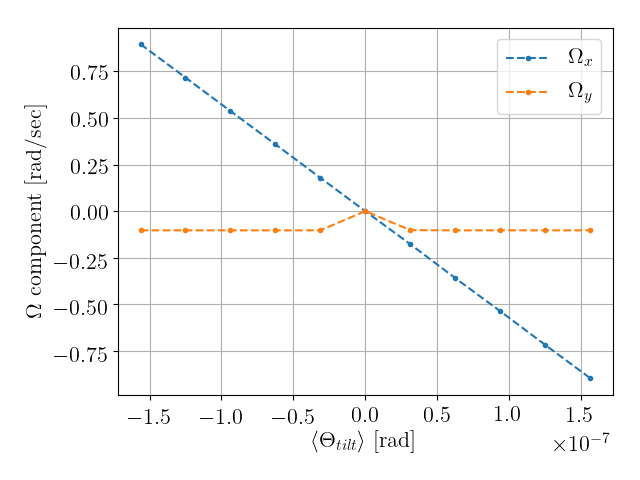
\includegraphics[height=.35\paperheight]{images/fake_signal_sim/linearity_test_compensated+microrad_freq}
		\caption{Angular velocity vector $\vec\W$ components.}
	\end{subfigure}
	\caption{Reference particle's spin precession axis and angular velocity components as
		functions of the mean E+B element tilt angle. Three mutually-compensated tilt pairs plus an uncompensated
		rotation.
		Color identifies the component; radial (blue) and vertical (orange)\label{fig:Linearity_test_compensated}}
\end{figure}

\subsection{Comparison of the CW vs CCW beams' spin precession angular velocities}\label{chpt3:imperfections:CW_vs_CCW}
In Figure~\ref{fig:Lin_test_rel_diff} we plotted the relative difference between the CW and CCW beams' radial SPA/angular velocity
components in the case of both the normally-distributed and mutually-compensated tilt cases.

For the raidal SPA component the relative difference was computed as
\[
\delta\bar n_x = \frac{\bar n_x^{CW}(\avg{\Theta_{tilt}}) - \bar n_x^{CCW}(\avg{\Theta_{tilt}})}{\bar n_x^{CW}(\avg{\Theta_{tilt}})};
\]
for the angular velocity:
\[
\delta\W_x = \frac{\W_x^{CW}(\avg{\Theta_{tilt}}) - \W_x^{CCW}(\avg{\Theta_{tilt}})}{\W_x^{CW}(\avg{\Theta_{tilt}})}.
\]

In the figures, one can observe that in either case both beams' SPA is oriented the same way; 
there is some difference between the beams' spin tunes, but it stays below the percent level. 
The spin tune difference grows bigger as the
spin wheel roll rate (proportional to the mean tilt angle) gets slower. 
The spin tune difference may indicate that
the lattice is asymmetric, with respect to the spin dynamics, relative to the beam circulation direction (i.e. time reversal).
It may be explained by a difference between the CW and CCW beams' closed orbits.

\begin{figure}[!h]
	\centering
	\begin{subfigure}{\linewidth}
		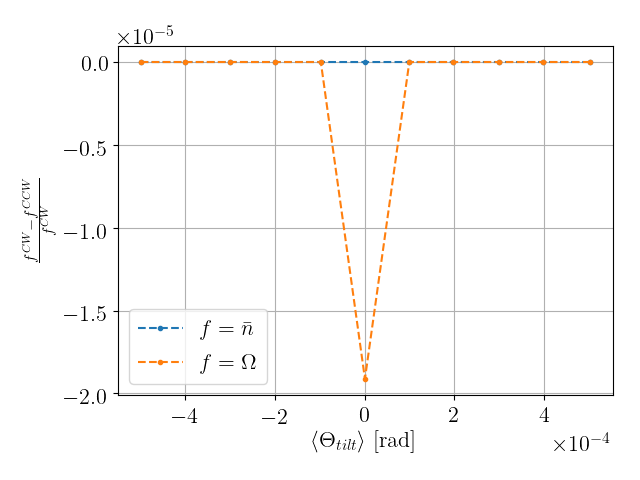
\includegraphics[height=.35\paperheight]{images/fake_signal_sim/linearity_test_shifting_gauss_rel_diff}	
		\caption{Normally distributed E+B element tilts.}
	\end{subfigure}
	\begin{subfigure}{\linewidth}
		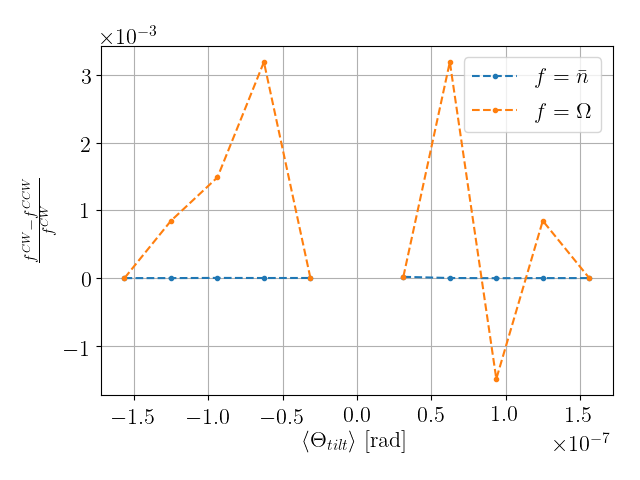
\includegraphics[height=.35\paperheight]{images/fake_signal_sim/linearity_test_compensated+microrad_rel_diff}
		\caption{Mutually-compensated element tilts.}
	\end{subfigure}
	\caption{Relative difference between the CW and CCW beams' spin precession axis and angular velocity radial components.
		Color marks the compared variable: spin precession axis (blue) and abgular velocity (orange).\label{fig:Lin_test_rel_diff}}
\end{figure}
